\subsection{可分超越基}

定义 1. --- 设 L 是域 K 的一个扩张。L 在 K 上的一个超越基 B 被称为可分的，如果 L 作为 K(B) 的代数扩张是可分的。

若 K 的特征为 0，则 L 在 K 上的每个超越基都是可分的，因为特征为 0 的域的每个代数扩张都是可分的（V，第 37 页，推论）。若一个扩张具有可分超越基，则它是可分的（V，第 121 页，命题 6 及第 122 页，命题 9）。下面的定理表明，每个有限生成的可分扩张都具有可分超越基；这一限制是本质的（V，第 177 页，习题 1）。

定理 5. --- 设 K 是一个域，L 是 K 的一个扩域，且 \((x_{i})_{i\in I}\) 是 L 的一个元素族。若该族 \((x_{i})_{i\in I}\) 是 L 在 K 上的一个可分超越基，则族 \((dx_{i})_{i\in I}\) 是向量空间 \(\Omega_{\mathrm{K}}(\mathrm{L})\) 在 L 上的一组基。若 L 是 K 的有限生成可分扩张，则逆命题成立。

令 \(\mathbf{M} = \mathbf{K}(x_i)_{i \in I}\) ，并用 \(\alpha\) 表示 \(\Omega_{\mathbf{K}}(\mathbf{M}) \otimes_{\mathbf{M}} \mathbf{L}\) 到 \(\Omega_{\mathbf{K}}(\mathbf{L})\) 中的典范映射。若 \((x_i)_{i \in I}\) 是 L 在 K 上的可分超越基，则族 \((d_{\mathbf{M}/\mathbf{K}} x_i)_{i \in I}\) 是向量 M-空间 \(\Omega_{\mathbf{K}}(\mathbf{M})\) 的一组基（V，第 128 页，命题 3），且 \(\alpha\) 是向量 L-空间的一个同构，因为 L 在 M 上是代数且可分的（V，第 130 页，推论 2）。由于 \(\alpha(d_{\mathbf{M}/\mathbf{K}} x_i \otimes 1) = d_{\mathbf{L}/\mathbf{K}} x_i\) ，族 \((d_{\mathbf{L}/\mathbf{K}} x_i)_{i \in I}\) 因此是 \(\Omega_{\mathbf{K}}(\mathbf{L})\) 在 L 上的一组基。

反之，假设 L 是 K 的一个可分有限生成扩张，并且族 \((d_{L/K}x_{i})_{i\in I}\) 是向量空间 \(\Omega_{K}(L)\) 在 L 上的一组基。由 V，第 134 页的推论 1，L 在 K 上的超越次数等于 \(\Omega_{K}(L)\) 在 L 上的维数，因此等于 I 的基数。由正合序列 \((\mathrm{E}_{\mathrm{K},\mathrm{M},\mathrm{L}})(\mathrm{V},\mathrm{p}.128)\) 我们有 \(\Omega_{\mathrm{M}}(\mathrm{L})=0\) ；由于 L 是 M 的有限生成扩张，V 第 135 页推论 2 表明 L 在 \(\mathbf{M}=\mathbf{K}(x_{i})_{i\in I}\) 上是代数且可分的；由于 L 在 K 上的超越次数是有限的且等于 I 的基数，族 \((x_{i})_{i\in I}\) 是 L 在 K 上的一个超越基（V，第 110 页，推论 1）。

推论. --- 设 L 是 K 的一个可分有限生成扩张，并设 S 是 L 的一个子集，使得 \(L = K(S)\) 。则存在 L 在 K 上的一个可分超越基 B，包含于 S 中。

由于 \(\Omega_{\mathrm{K}}(\mathrm{L})\) 由 S 中元素的微分生成，存在 S 的 s 个元素 \(x_{1}, \ldots, x_{s}\) ，使得 \((dx_{1}, \ldots, dx_{s})\) 是 \(\Omega_{\mathrm{K}}(\mathrm{L})\) 在 L 上的一组基。现在只需应用定理 5。

注记. --- 设 L 是特征为 \(p \neq 0\) 的域 K 的一个可分有限生成扩张；可能存在 L 的并非可分的超越基。只需观察到 \(\{X^{p}\}\) 是 \(\mathrm{K}(\mathbf{X})\) 的一个超越基，但 \(\mathrm{K}(\mathbf{X})\) 是 \(\mathrm{K}(\mathbf{X}^{p})\) 的次数为 p 的 p-根式扩张。

命题 5. --- 设 L 和 M 是域 K 的两个扩张，包含于一个给定的扩张中，且在 K 上代数不相交。若 M 在 K 上可分，则 L(M) 在 L 上可分。

只需证明对于 M 的每个有限子集 S，L(S) 在 L 上可分即可（V，第 122 页，命题 8）。设 S 为 M 的有限子集。由于域 K(S) 在 K 上可分，故其具有可分超越基 B（定理 5 的推论）。由于 L 与 M 在 K 上代数不相交，B 是 L(B) 在 L 上的超越基（V，第 113 页，命题 12）。进一步，S 的每个元素在 K(B) 上都是代数且可分的，因此在 L(B) 上亦然（V，第 39 页，推论 2）。我们由此推出（V，第 39 页，命题 6）L(S) = L(B)(S) 在 L(B) 上是代数且可分的，因此 L(S) 在 L 上可分。

推论. --- 若 L 与 M 是 K 上可分且代数不相交的扩张，则域 \(\mathbf{K}(\mathbf{L} \cup \mathbf{M})\) 在 K 上是可分的。

由于 \(K(L \cup M) = L(M)\) 由命题 5 在 L 上是可分的（因为 M 在 K 上是可分的），且 L 在 K 上是可分的，故得推论（V，第 122 页，命题 9）。

\pandocbounded{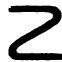
\includegraphics[keepaspectratio]{images/part002_2c83366d.jpg}}

L 和 M 的扩张在代数上不相交这一假设在命题 5 及其推论中是必不可少的。因为设 K 是一个特征为 \(p \neq 0\) 的非完全域，E 是形如 \(\mathrm{K}(x, a)\) 的扩张，其中 x 在 K 上超越，a 是 K 上高度为 1 的 p-根式元；令 \(\mathrm{L} = \mathrm{K}(x)\) 且 \(\mathrm{M} = \mathrm{K}(x + a)\) 。则 \(x + a\) 在 K 上超越（若非如此， \(x = (x + a) - a\) 将在 K 上代数），且域 L 与 M 在 K 上可分。然而， \(\mathrm{K}(\mathrm{L} \cup \mathrm{M}) = \mathrm{K}(x, a)\) 是 \(\mathrm{L} = \mathrm{K}(x)\) 上的次数为 p 的 p-根式扩张，且在 L 上不可分，在 K 上也不可分。

